\chapter{Perfiles de estudiantes según su rendimiento}
\addcontentsline{toc}{chapter}{Perfiles de estudiantes según su rendimiento}

Debido a la dificultad de predecir de manera exacta la calificación obtenida por los alumnos a partir de las medidas de rendimiento descritas anteriormente, se agruparán las notas en clusters significativos y trataremos de predecir en qué cluster se encuentra la nota de un determinado grupo de alumnos.

\section{Por clusters fijos de notas}

En primer lugar, escogeremos como separación los cuartiles de las calificaciones. Así pues, podemos ver la distribución de los cuartiles en la Figura \ref{fig:boxplotquartilegrade}, donde los límites inferiores de cada una de las cajas son $6.99$, $8.23$, $8.95$ y $9.60$ respectivamente. También puede verse en la Figura \ref{fig:countquartilegrade} el número de grupos que hay en cada cuartil.


\begin{figure}[H]
\centering
\subfloat[Boxplot de las calificaciones por cuartil.]{\label{fig:boxplotquartilegrade}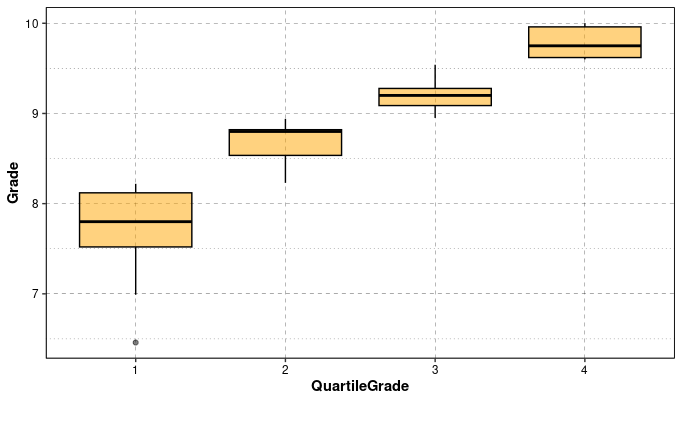
\includegraphics[width=0.47\textwidth]{clustering/boxplotgrade.png}}\qquad
\subfloat[Número de grupos por cuartil.]{\label{fig:countquartilegrade}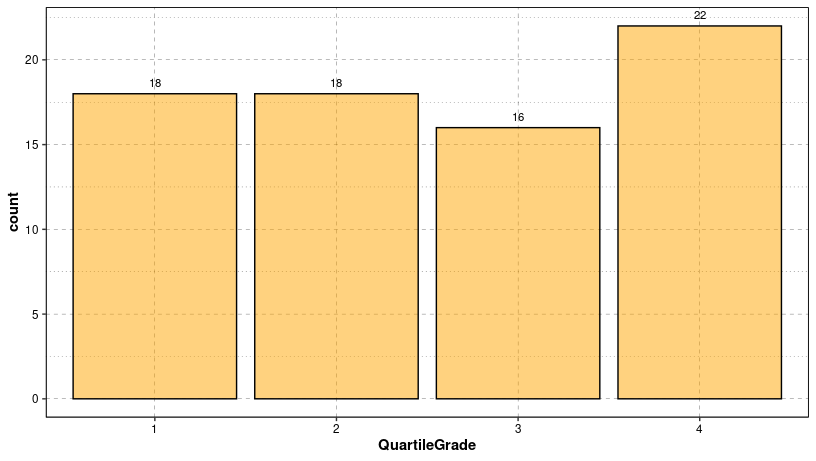
\includegraphics[width=0.47\textwidth]{clustering/countquartilegrade.png}}%
\caption{Resultados obtenidos tras aplicar el algoritmo agrupar las caficaciones por cuartiles.}
\label{fig:quartilegradeclustering}
\end{figure}

Sin embargo, en la Figura \ref{fig:boxplotquartilegrade} y en la Figura \ref{fig:frequenciesgrade}, donde se representan cómo de frecuentes son cada una de las calificaciones obtenidas, notamos la presencia de un outlier.

\begin{figure}[H]
    \centering
    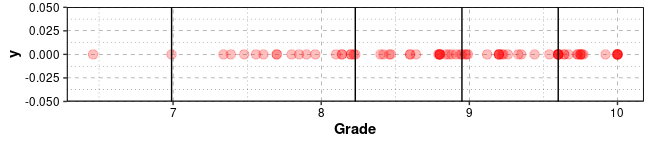
\includegraphics[width=0.6\textwidth]{clustering/frequencygrade.png}
    \caption{Calificaciones obtenidas por los distintos grupos. El límite de los cuartiles se ha indicado con líneas verticales negras.}
    \label{fig:frequenciesgrade}
\end{figure}

En la Figura \ref{fig:densitybyfactorquartilegrade} vemos las funciones de densidad por cuartil. Prestaremos especial atención a los grupos del cluster \texttt{Q1} (el de las peores calificaciones al que le añadimos el outlier) puesto que son los que peor rendimiento han mostrado.

\begin{figure}[H]
    \centering
    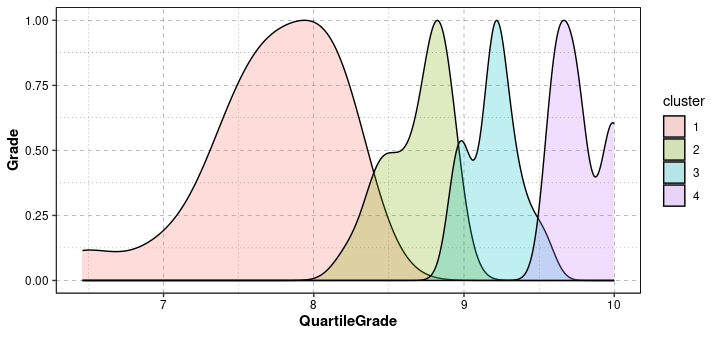
\includegraphics[width=0.6\textwidth]{clustering/densitybyfactorquartilegrade.png}
    \caption{Funciones de densidad de las calificaciones obtenidas por cluster.}
    \label{fig:densitybyfactorquartilegrade}
\end{figure}

\section{Por clusters dinámicos de notas}

Se agruparán los datos usando el algoritmo de las K-medias sobre la variable \emph{Grade}. Para decidir el número de clusters en el que agruparemos los datos, se usarán métodos gráficos. Como podemos ver en las Figuras \ref{fig:indiceshubert} y \ref{fig:indicesdindex}, el número óptimo de particiones podría ser $3$ o $5$. Para decidir entre un número de clusters u otro se realizarán los dos agrupamientos y nos quedaremos con el de menor error.

\begin{figure}[H]
    \centering
    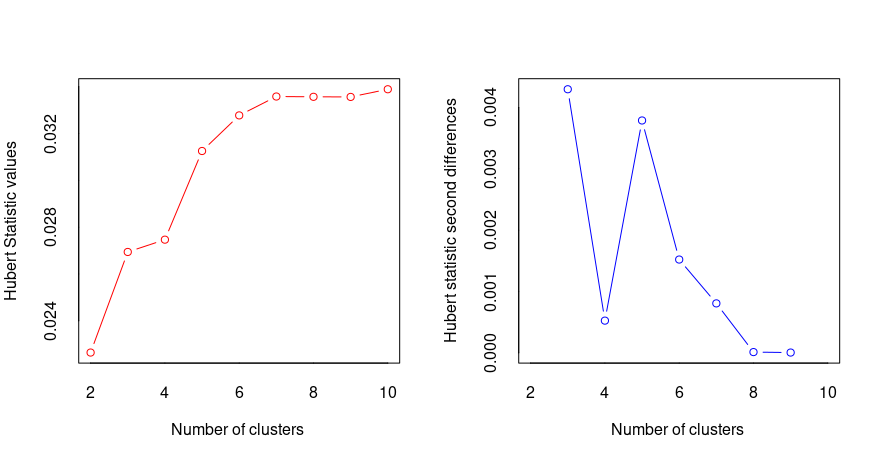
\includegraphics[width=\textwidth]{clustering/Hubert.png}
    \caption{Valores estadísticos de Hubert.}
    \label{fig:indiceshubert}
\end{figure}

\begin{figure}[H]
    \centering
    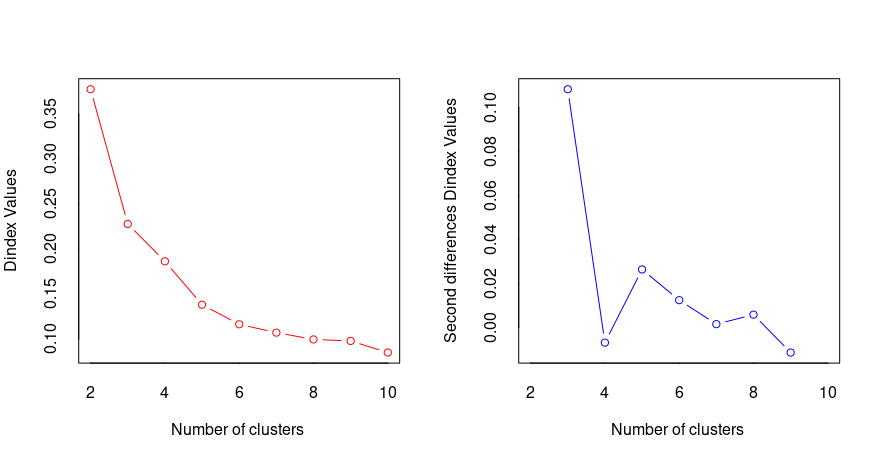
\includegraphics[width=\textwidth]{clustering/Dindex.png}
    \caption{Valores de Dindex.}
    \label{fig:indicesdindex}
\end{figure}

Aplicando el algoritmo de las K-medias para $K = 2$ (Figura \ref{fig:KMeans2}) y para $K = 3$ (Figura \ref{fig:KMeans3}), vemos que hay una gran diferencia la precisión de uno y otro (para $K = 2$ se tiene $\texttt{accuracy} = 0.6978412$ mientras que para $K = 3$ (Figuras) se tendrá $\texttt{accuracy} = 0.8585982$). Como podemos ver en la Figura \ref{fig:KMeans2}, seguimos teniendo un outlier.

\begin{figure}[H]
    \centering
    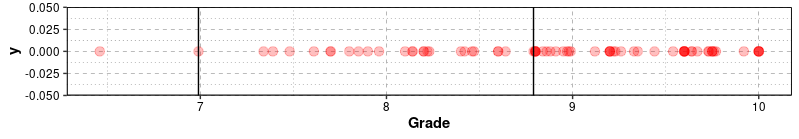
\includegraphics[width=0.6\textwidth]{clustering/KMeans2.png}
    \caption{Particiones obtenidas con $K = 2$.}
    \label{fig:KMeans2}
\end{figure}

\begin{figure}[H]
    \centering
    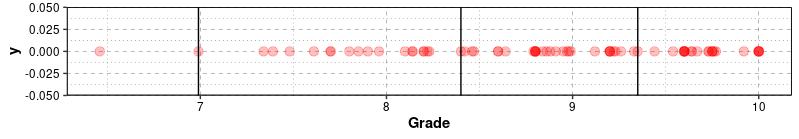
\includegraphics[width=0.6\textwidth]{clustering/KMeans3.png}
    \caption{Particiones obtenidas con $K = 3$.}
    \label{fig:KMeans3}
\end{figure}

La distribución de la variable \emph{Grade} dentro de cada partición puede verse en las Figuras \ref{fig:KMeans2boxplot} y \ref{fig:KMeans3boxplot} mientras que el número de grupo que hay en las particiones puede verse en las Figuras \ref{fig:KMeans2count} y \ref{fig:KMeans3count}.

\begin{figure}[H]
\centering
\subfloat[Boxplot de cada una de las particiones.]{\label{fig:KMeans2boxplot}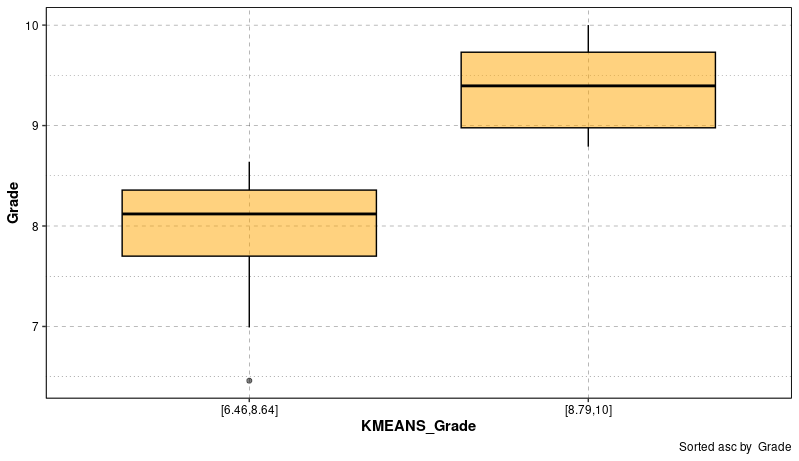
\includegraphics[width=0.47\textwidth]{clustering/KMeans2boxplot.png}}\qquad
\subfloat[Número de grupos por partición.]{\label{fig:KMeans2count}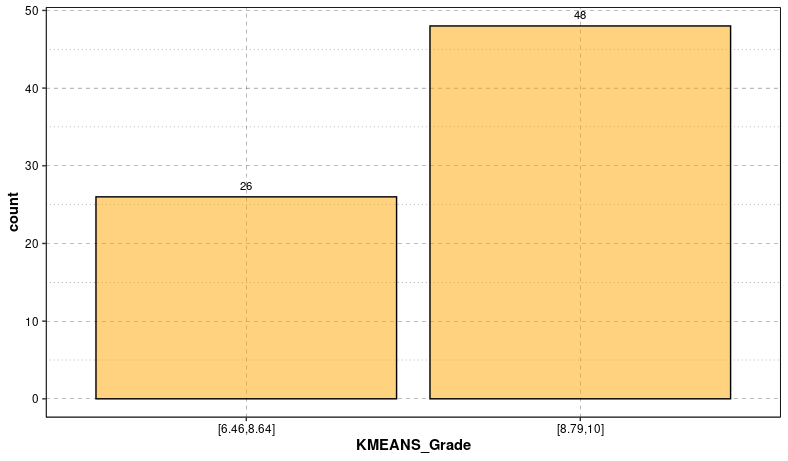
\includegraphics[width=0.47\textwidth]{clustering/KMeans2count.png}}%
\caption{Resultados obtenidos tras aplicar el algoritmo de las $K$-Medias con $K = 2$.}
\label{fig:KMeans2details}
\end{figure}

\begin{figure}[H]
\centering
\subfloat[Boxplot de cada una de las particiones.]{\label{fig:KMeans3boxplot}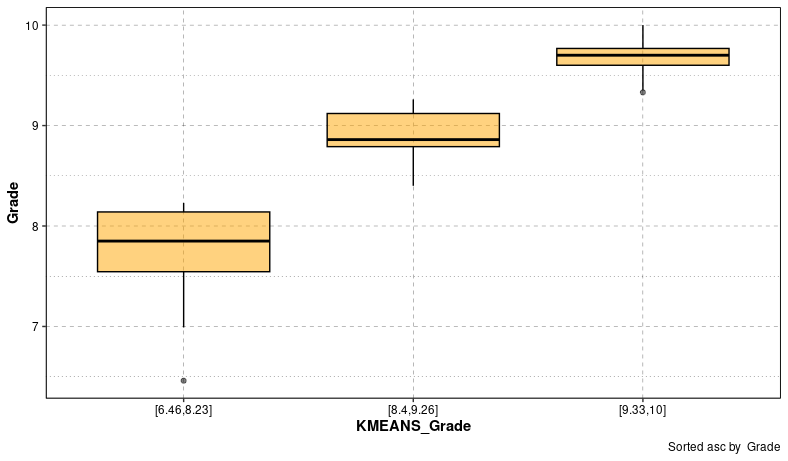
\includegraphics[width=0.47\textwidth]{clustering/KMeans3boxplot.png}}\qquad
\subfloat[Número de grupos por partición.]{\label{fig:KMeans3count}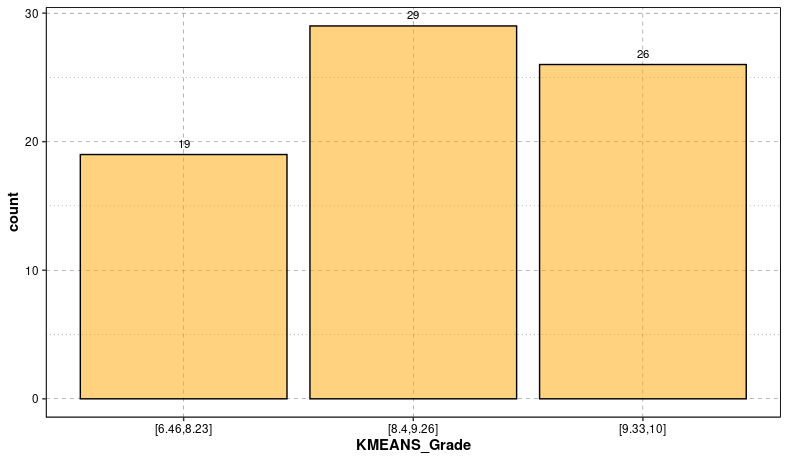
\includegraphics[width=0.47\textwidth]{clustering/KMeans3count.png}}%
\caption{Resultados obtenidos tras aplicar el algoritmo de las $K$-Medias con $K = 3$.}
\label{fig:KMeans3details}
\end{figure}

Por último, para cinco particiones (Figura \ref{fig:KMeans5}) se tendrá $\texttt{accuracy} = 0.9474439$. Es decir, tenemos más precisión con cinco particiones y ya no tenemos outliers. Nos centramos en estudiar los grupos de los dos primeros clusters (aquellos grupos con una nota inferior a $7.34$).

\begin{figure}[H]
    \centering
    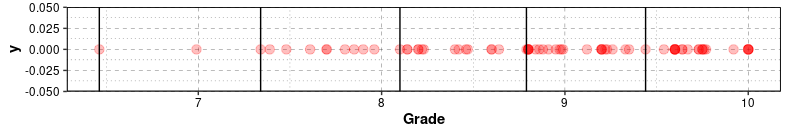
\includegraphics[width=0.6\textwidth]{clustering/KMeans5.png}
    \caption{Particiones obtenidas con $K = 5$.}
    \label{fig:KMeans5}
\end{figure}

\begin{figure}[H]
\centering
\subfloat[Boxplot de cada una de las particiones.]{\label{fig:KMeans5boxplot}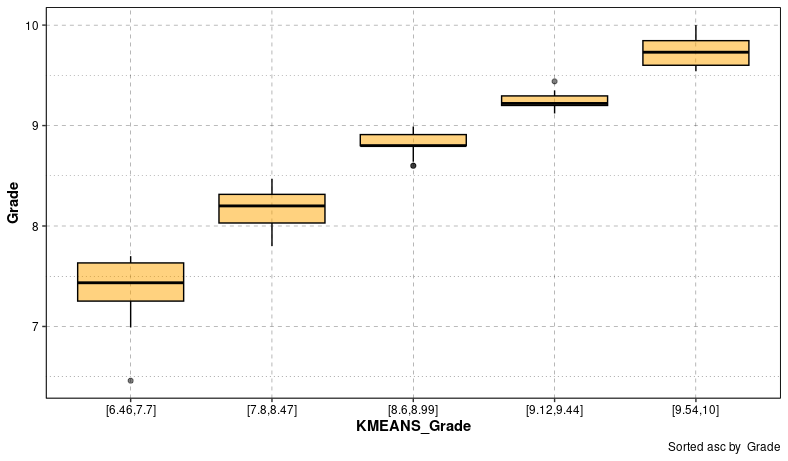
\includegraphics[width=0.47\textwidth]{clustering/KMeans5boxplot.png}}\qquad
\subfloat[Número de grupos por partición.]{\label{fig:KMeans5count}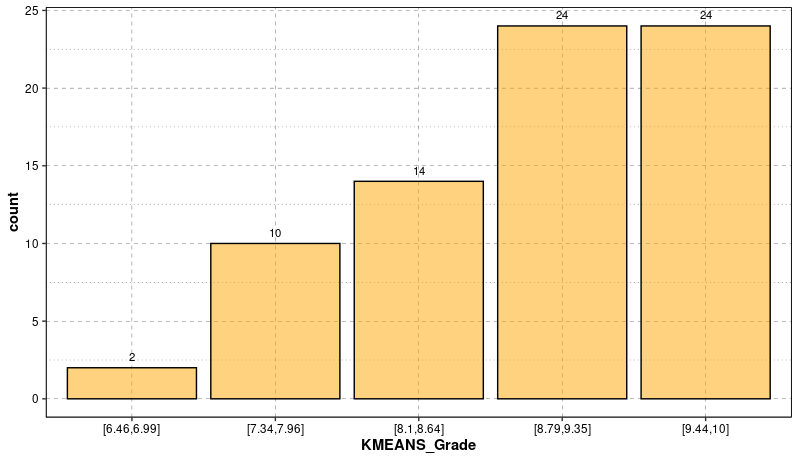
\includegraphics[width=0.47\textwidth]{clustering/KMeans5count.png}}%
\caption{Resultados obtenidos tras aplicar el algoritmo de las $K$-Medias con $K = 5$.}
\label{fig:KMeans5details}
\end{figure}

\section{Por clusters aproximados de rendimiento}

De las medidas de rendimiento estudiadas en la sección \textbf{Incluir referencia}, nos quedaremos con aquellas que correlan con la variable \emph{Grade}.